\documentclass[a4paper,twoside,listof=totoc]{scrbook}

% Language support
\usepackage[magyar]{babel}

% Page geometry
\usepackage[
  top=1in,
  bottom=1in,
  inner=.8in,
  outer=1.2in,
  footskip=.5in,
]{geometry}

% Document title, author
\usepackage{fontawesome}
\title{
  Rendszer- és irányítástechnika \\
  szóbeli tételsor

}
\author{Sándor Tibor}
\date{
  \today \\
  % (1 $\faSpinner$, 2 $\times$)\\
  \texttt{v1.1.0} \\
}

% Page style
\usepackage[
  luatex,
  colorlinks=true,
  allcolors=darkRed
]{hyperref}
\usepackage{fancyhdr}
\usepackage{lastpage}
\pagestyle{fancy}
\renewcommand{\headrulewidth}{2pt}
\renewcommand{\footrulewidth}{2pt}
\fancyfoot[RO,LE]{\thepage}
\fancyfoot[RE,LO]{\textit{Készítette:} Sándor Tibor}
\fancyfoot[C]{}
\fancyhead[RO,LE]{\textsl{\nouppercase{\rightmark}}}
\fancyhead[RE,LO]{\textsl{\nouppercase{\leftmark}}}

\renewcommand{\chaptermark}[1]{%
  \markboth{\thechapter\ #1}{}
}
\renewcommand{\sectionmark}[1]{%
  \markright{\thesection\ #1}{}
}

% Head and foot rule width
\renewcommand{\headrulewidth}{1pt}
\renewcommand{\footrulewidth}{1pt}

% Paragraph spacing
\setlength{\parindent}{0em}
\setlength{\parskip}{.5em}

% Colorful 'titles'
\setkomafont{disposition}{\color{darkRed}\bfseries\sffamily}
\setkomafont{captionlabel}{\color{darkRed}\bfseries\sffamily}
\renewcommand{\theequation}{{\bfseries\color{darkRed}\thesection.\arabic{equation}}}

% Basic math packages
\usepackage{fontspec}
\usepackage{amsmath}
\usepackage{amssymb}
\usepackage{unicode-math}

\setmainfont{TeX Gyre Pagella}
\setmathfont{TeX Gyre Pagella Math}
% \setmathfont{Asana Math}
\setsansfont[Scale=MatchUppercase]{TeX Gyre Heros}
\everydisplay{\Umathoperatorsize\displaystyle=5ex}

% Equation numbreing as (s.ss)
\counterwithout{section}{chapter}
\numberwithin{equation}{section}
\renewcommand{\theequation}{{\bfseries\color{darkRed}\thesection.\arabic{equation}}}

% Very important for variable printing
\usepackage{icomma}
\usepackage[
  locale=DE,
  per-mode=symbol
]{siunitx}

% Graphics
\usepackage{tikz}
\usetikzlibrary{
  calc,
  decorations.pathreplacing,
  calligraphy
}
\usepackage{pgfplots}
\pgfplotsset{compat=newest}
\usepackage{bodeplot}
\pgfkeys{/pgf/plot/gnuplot call={cd build && gnuplot}}

% Other packages
\usepackage{tabto}
\usepackage{multicol}
\usepackage{float}
\usepackage{caption}
\usepackage{subcaption}
\usepackage{standalone}
\usepackage{xfrac}
\usepackage{bm}
\usepackage{arydshln}
\usepackage{enumitem}

% Math custom commands
\newcommand\iu{\symbf{j}}
\newcommand{\rvec}[1]{\mathbfit{#1}}
\newcommand{\tvec}[1]{\tilde{\mathbfit{#1}}}
\newcommand{\uvec}[1]{\widehat{\mathbfit{#1}}}
\newcommand{\hvec}[1]{\hat{\mathbfit{#1}}}
\newcommand{\rmat}[1]{\symbf{#1}}
\newcommand{\tmat}[1]{\tilde{\symbf{#1}}}
\newcommand{\hmat}[1]{\hat{\symbf{#1}}}
\newcommand{\abs}[1]{\left|#1\right|}
\newcommand{\dirac}{\delta}
\newcommand{\step}{\varepsilon}
\newcommand{\Imat}{\mathbb{I}}
\newcommand{\nvec}{\bm{\mathit 0}}
\newcommand{\e}{\mathbb e}
\newcommand{\T}{\mathsf T}

\DeclareMathOperator\sgn{sgn}
\DeclareMathOperator\adj{adj}
\DeclareMathOperator\rank{rank}

\makeatletter
\DeclareRobustCommand*{\slashfracstyle}[1]{%
  {\m@th\ensuremath{\mbox{\fontsize\sf@size\z@\selectfont #1}}}}
\DeclareRobustCommand*{\slashfrac}[2]{\leavevmode
  \raise.25ex\hbox{\slashfracstyle{#1}}\kern-.075em/%
  \kern-.075em\lower.25ex\hbox{\slashfracstyle{#2}}}
\makeatother

% Custom inputs
\usepackage{xcolor}
\colorlet{darkRed}{red!40!black}
\colorlet{darkBlue}{cyan!50!black}
\colorlet{darkYellow}{yellow!50!black}

\newenvironment{about}{\color{darkBlue!40!gray!80}\sffamily\large}{\ignorespacesafterend\par}


% Document starts here
\begin{document}

% \frontmatter

\vbox{
  \maketitle

  % \vspace{4cm}
  %
  % \centering
  % \includestandalone{./graphics/title_graphics}
}

\tableofcontents
\begingroup
\vfill
\let\cleardoublepage\relax
\listoffigures
\endgroup

% \mainmatter

\chapter{Klasszikus szabályozáselmélet}
% \thispagestyle{fancy}

\section{Kanonikus szabályozási kör felépítése}

\begin{about}
  Ismertesse a kanonikus szabályozási kör elvi felépítését, egy példán
  keresztül mutassa be az arányos (P), az integráló (I) és a deriváló (D) tagok
  szerepét a szabályozási körben!
\end{about}

\subsection{A szabályozási kör felépítése}

\begin{figure}[htb]
  \centering
  \includestandalone{../graphics/control_loop_text}
  \caption{A szabályozási kör elvi felépítése}
  \label{fig:control-loop-text}
\end{figure}

A szabályozási kör három szakaszból épül fel: a szabályozóból, a szabályozott
szakaszból, valamint a visszacsatoló tagból.
Egy ilyen rendszertől elvárjuk, hogy stabil és megvalósítható legyen.
A statikus pontosság (alapjelkövetés), zavar-kompenzáció és zajelnyomás is
fontos követelmény.

\begin{figure}[htb]
  \centering
  \includestandalone{../graphics/control_loop_basic}
  \caption{A szabályozási kör elvi felépítése}
  \label{fig:control-loop-basic}
\end{figure}

Tanulmányaink során SISO (Single Input Single Output / 1 bemenet 1 kimenet)
rendszerekkelfoglalkoztunk. A visszacsatoló hatást konstans egynek vettük, a
zajt és a zavarást pedig a legtöbb esetben elhanyagoltuk. A szabályozási kör
hatásvázlata ilyen esetben a \ref{fig:control-loop-basic}. ábrán látható.

\subsection{Arányos (P) tag hatása}

Alkalmazzunk arányos szabályozó tagot egy olyan szakaszon, melynek átviteli
függvénye egytárolós jellegű vagyis:
\begin{equation}
  W_c(s) = P,
  \quad \text{ és } \quad
  W_p(s) = \frac{A}{1 + sT}
  .
  \label{eq:P-use-CP}
\end{equation}
Ekkor a referenciajel és a kimenet közötti árviteli függvény:
\begin{equation}
  W_{cl}(s)
  = \frac{W_o}{1 + W_o}
  = \frac{PA / (1 + sT)}{1 + PA / (1 + sT)}
  = \frac{PA}{1 + sT + PA}
  = \frac{(PA) / (1 + PA)}{1 + (sT) / (1 + PA)}
  = \frac{\tilde A}{1 + s \tilde T}
  .
  \label{eq:P-use-cl}
\end{equation}

Az arányos taggal tehát gyorsítani tudjuk a rendszerünket, hiszen a jól
megválasztott $P$ taggal a rendszer időállandója csökkenthető. Ennek hatására
megváltozik viszont a rendszer erősítése is, maradó hibája lesz a kimenetnek,
méghozzá $e(\infty) = 1 - \tilde A$ nagyságú. Ezt a hibát statikus
alapjel-kompenzációval kiküszöbölhetjük. A referencia jelet egy $W_f(s) = 1 /
  \tilde A$ átviteli függvénnyel rendelkező arányos tagon kell átvezetni annak
érdekében, hogy a maradó hiba zérus legyen. A rendszer válasza ekkor
egységugrásra:
\begin{equation}
  v(t)
  = \frac{1}{\tilde A} \cdot \tilde A \left( 1 - e^{\slashfrac{-t}{T}} \right)
  = 1 - e^{\slashfrac{-t}{T}}
  \label{eq:P-use-step}
\end{equation}

\subsection{Integráló (I) tag hatása}

Alkalmazzunk most I szabályozót az előző alfejezetben bemutatott egytárolós
szakaszon. Ekkor az átviteli függvények:
\begin{equation}
  W_c(s) = \frac{I}{s},
  \quad \text{ és } \quad
  W_p(s) = \frac{A}{1 + sT}
  .
  \label{eq:I-use-CP}
\end{equation}
A referenciajel és a kimenet közötti árviteli függvény:
\begin{equation}
  W_{cl}(s)
  = \frac{AI}{s(1 + sT) + AI}
  = \frac{AI}{s^2 T + s + AI}
  = \frac{AI / T}{s ^ 2 + s / T + AI / T}
  = \frac{\omega_n^2}{s^2 + 2 \zeta \omega_n s + \omega_n^2}
  .
  \label{eq:I-use-cl}
\end{equation}

Látható, hogy a rendszer sajátkörfrekvenciája ($\omega_n = \sqrt{AI / T}$) és
csillapítása ($\zeta = 1 / (2 T \omega_n)$) az $I$ paraméter
megválasztásával beállítható. Ezek a rendszer további minőségi jellemzőit
is meg fogják határozni. A rendszer válasza egységugrásra ($\zeta^2 < 1$ --
alulcsillapítás esetén):
\begin{equation}
  v(t)
  = 1 - e^{-\zeta \omega_n t} \left(
  \cos \omega_d t + \frac{\zeta}{\sqrt{1 - \zeta^2}}  \sin \omega_d t
  \right)
  .
  \label{eq:I-use-step}
\end{equation}

\subsection{Deriváló (D) tag hatása}

Alkalmazzunk most egy D tagot egy kéttárolós tag esetén. Ekkor az átviteli
függvények:
\begin{equation}
  W_c(s) = Ds,
  \quad \text{ és } \quad
  W_p(s) = \frac{A}{s (1 + sT)}
  .
  \label{eq:D-use-CP}
\end{equation}

Hatása hasonló a $P$ tag hatásáéhoz, itt is maradó hiba keletkezik, úgyhogy
önmagában nem alkalmazható.

\section{Stabilitás kritériumok}

\begin{about}
  Mutassa be lineáris időinvariáns rendszerekre vonatkozóan az alapvető
  stabilitási definíciókat (BIBO stabilitás fogalma, magára hagyott rendszer
  stabilitása) és azok kritériumait (Routh-Hurwitz stabilitási kritérium, Bode
  stabilitási kritérium) szabályozási körökre alkalmazva!
\end{about}

A lineáris, időinvariáns rendszerekre jellemző, hogy érvényes rájuk a
szuperpozíció elve, valamint ugyanarra a bemenetre időponttól függetlenül
ugyanolyan választ adnak.

\subsection{BIBO stabilitás}

A BIBO (Bounded Input -- Bounded Output / Gerjesztés -- Válasz) stabilitási
feltétel azt vizsgálja, hogy véges bemenetre adott válasz véges kimenetet
eredményez-e. A bemenet korlátos, ha $\abs{u(t)} \leq A < \infty$
egyenlőtlenség fennáll, valamint azt is tudjuk, hogy az operátor tartományban
végzett szorzás időtartományban konvolúciós integrálással ekvivalens.
Laplace-tartományban a kimenet a bemenet és az átviteli függvény szorzataként
áll elő, ezért $t$ tartományban a kimenet az alábbi alakban írható fel:
\begin{equation}
  y(t)
  = \int_0^\infty w(\tau) \cdot u(t - \tau) \, \mathrm d t.
  \label{eq:BIBO-conv}
\end{equation}
Majoráljuk a kimenet abszolút értékét az alábbi módon:
\begin{equation}
  \abs{y(t)}
  = \abs{\int_0^\infty w(\tau) \cdot u(t - \tau) \, \mathrm d t}
  \leq \int_0^\infty \abs{w(\tau)} \cdot \abs{u(t - \tau)} \, \mathrm d t
  \leq A \int_0^\infty \abs{w(\tau)} \, \mathrm d t.
  \label{eq:BIBO-major}
\end{equation}
Látható, hogy ha a rendszer $w(t)$ súlyfüggvénye lecsengő, állandósult értéke
zérus, akkor az alábbi improprius integrál konvergens, a kimenet ebből
következően véges lesz.

\subsection{Magára hagyott rendszer stabilitása}

\begin{figure}[htb]
  \centering
  \includestandalone{../graphics/asymptotic}
  \caption{
    A rendszer stabilitása valós és komplex pólusok esetén
    ({\color{darkBlue} stabil},
    {\color{darkYellow} határhelyzet},
    {\color{darkRed} instabil})
  }
  \label{fig:asymptotic-poles}
\end{figure}
Az aszimptotikus stabilitási feltétel (magára hagyott rendszer stabilitása)
azt vizsgálja meg, hogy a nyugalmi helyzetéből kimozdított rendszer visszatér-e
az egyensúlyi helyzetébe, ha a rendszert a kimozdítás után magára hagyjuk.

A szabályozott szakasz átviteli függvénye felírható az alábbi alakban:
\begin{equation}
  W_{cl}(s)
  = \frac{W_c(s) W_p(s)}{1 + W_c(s) W_p(s)}
  = \frac{W_o(s)}{1 + W_o(s)}
  = \frac{N_o / D_o}{1 + N_o / D_o}
  = \frac{N_o}{N_o + D_o}
  .
  \label{eq:asymptotic-cl}
\end{equation}
Készítsünk karakterisztikus polinomot, amely $N_o$ és $D_o$ polinomok
összegeként állítunk elő. Vizsgáljuk meg ezen polinom gyökeit. Megállapíthatjuk,
hogy amennyiben a gyökök valós részei negatívok, akkor a rendszer stabil lesz,
a kimenet állandósult értéke zérus.

\subsection{Routh-Hurwitz stabilitási kritérium}

A $p(s) = N_o + D_o$ karakterisztikus polinom gyökei bizonyos fokszám fölött
nehezen határozhatóak meg. Ilyen esetben alkalmazhatjuk a Routh-Hurwitz
kritériumot. Hozzuk a karakterisztikus polinomot az alábbi alakra:
\begin{equation}
  p(s) = a_n s^n + a_{n-1} s^{n-1} + \dots + a_1 s + a_0.
  \label{eq:RH-poles}
\end{equation}

A stabilitás szükséges feltétele, hogy a polinom együtthatói azonos előjelűek
legyenek, vagyis $\sgn a_0 = \sgn a_1 = ... = \sgn a_n$.

A stabilitás elégséges feltétele pedig, hogy a Hurwitz-mátrix minden egyes
főátlójára feszített aldeterminánsa azonos előjelű legyen. Ezen mátrix az
alábbi alakban írható fel:
\begin{equation}
  \rmat H = \begin{bmatrix}
    a_{n-1} & a_{n-3} & a_{n-5} & \hdots & 0      \\
    a_{n}   & a_{n-2} & a_{n-4} & \hdots & 0      \\
    0       & a_{n-1} & a_{n-3} & \hdots & 0      \\
    \vdots  & \vdots  & \vdots  & \ddots & \vdots \\
    0       & 0       & 0       & \hdots & a_0    \\
  \end{bmatrix}
  .
  \label{eq:RH-matrix}
\end{equation}

\subsection{Bode stabilitási kritérium}

\begin{figure}[htb]
  \centering
  \hspace{-4cm}
  \includestandalone{../graphics/bode-PM}
  \caption{Rendszer {\color{darkRed} fázis}- és {\color{darkYellow} erősítés}tartaléka}
  \label{fig:Bode-PM}
\end{figure}

A stabilitás vizsgálatot a Bode-diagram alapján is elvégezhetjük. Vizsgáljuk
a felnyitott kör átviteli függvényét. Éljünk az $s = \iu \omega$ formális
helyettesítéssel. Keressük meg $\omega_c$ vágási körfrekvenciát, ahol az
erősítés egységnyi ($\abs{W_o(\iu \omega_c)} = A(\omega_c) = 1 = 0 \,
  \mathrm{dB}$). Számítsuk ki a fázistartalékot az alábbi képlettel:
\begin{equation}
  \varphi_t = \varphi(\omega_c) - (- \pi)
  .
  \label{eq:Bode-PM}
\end{equation}
Amennyiben a fázistartalék pozitív, a rendszer stabil.

\section{Kanonikus szabályozási kör elvi felépítése}

\begin{about}
  Ismertesse a kanonikus szabályozási kör elvi felépítését, mutassa be az
  alapjel, a zavarás és a zaj hatását, mint a rendszer bemenetei a kimenő jelre,
  a hibajelre és a beavatkozó jelre, mint a rendszer kimenetei!
\end{about}

\begin{figure}[htb]
  \centering
  \includestandalone{../graphics/control_loop_disturbances}
  \caption{A szabályozási kör zavarásokkal, zajjal kiegészítve}
  \label{fig:control-loop-disturbances}
\end{figure}

\begin{multicols}{2}
  A szabályozási kör bemenetei:
  \begin{itemize}
    \item $R(s)$ -- referenciajel,
    \item $D_i(s)$ -- bemeneti zavarás,
    \item $D_o(s)$ -- kimeneti zavarás,
    \item $N(s)$ -- zaj.
  \end{itemize}

  A szabályozási kör kimenetei:
  \begin{itemize}
    \item $Y(s)$ -- kimenőjel,
    \item $E(s)$ -- hibajel,
    \item $U(s)$ -- beavatkozó jel.
  \end{itemize}
\end{multicols}

A bemenetek hatása a kimenőjelre:
\begin{equation}
  Y(s)
  = \left( \frac{W_c W_p} {1 + W_o} \right) R(s)
  + \left( \frac{W_p}     {1 + W_o} \right) D_i(s)
  + \left( \frac{1}       {1 + W_o} \right) D_o(s)
  + \left( \frac{-W_c W_p}{1 + W_o} \right) N(s)
  .
  \label{eq:disturbances-Y}
\end{equation}

A bemenetek hatása a beavatkozó jelre:
\begin{equation}
  U(s)
  = \left( \frac{W_c}     {1 + W_o} \right) R(s)
  + \left( \frac{-W_o}    {1 + W_o} \right) D_i(s)
  + \left( \frac{-W_c W_v}{1 + W_o} \right) D_o(s)
  + \left( \frac{-W_c}    {1 + W_o} \right) N(s)
  .
  \label{eq:disturbances-U}
\end{equation}

A bemenetek hatása a hibajelre:
\begin{equation}
  E(s)
  = \left( \frac{1}       {1 + W_o} \right) R(s)
  + \left( \frac{-W_p W_v}{1 + W_o} \right) D_i(s)
  + \left( \frac{-W_v}    {1 + W_o} \right) D_o(s)
  + \left( \frac{-1}      {1 + W_o} \right) N(s)
  .
  \label{eq:disturbances-E}
\end{equation}

A korábbi egyenletekben $W_o(s)$ a felnyitott kör átviteli függvénye, amely
az alábbi módon számítható:
\begin{equation}
  W_o(s) = W_c(s) W_p(s) W_v(s)
  .
  \label{eq:disturbances-o}
\end{equation}

Számításaink során gyakran egyszerűsítéseket teszünk. Elhanyagoljuk a kimeneti
zavarást, $W_v(s)$ függvény értékét pedig egységnyinek válasszuk meg.
Ebben az esetben a kimenet és a referenciajel között felírt átviteli függvény --
melyet gyakran a zárt szabályozási kör átviteli függvényének is nevezünk --
az alábbi alakra redukálódik:
\begin{equation}
  W_{cl}
  = \frac{W_c W_p}{1 + W_c W_p}
  = \frac{W_o}{1 + W_o}
  .
  \label{eq:disturbances-cl}
\end{equation}

\section{PI és PD szabályozók}

\begin{about}
  Ismertesse a PI és PD szabályozó egyenletét idő és operátor tartományban!
  Mutassa be a pólus-zérus kiejtésen alapuló szabályozótervezés menetét!
  Válaszában térjen ki az ideális és a megvalósítható deriváló (D) tagok
  összefüggésére is!
\end{about}

\subsection{P, I és D tagok egyenletei}

% \subsubsection{P tag}

Az \textbf{arányos tag} operátor tartománybeli egyenlete: $W(s) = P$.
Idő tartománybeli ugrás válasza:
\begin{equation}
  v(t) = \mathcal{L}^{-1} \{ P / s \} = P.
  \label{eq:P-step}
\end{equation}

% \subsubsection{I tag}

Az \textbf{integráló tag} operátor tartománybeli egyenlete: $W(s) = I/s$.
Ugrás válasza:
\begin{equation}
  v(t) = \mathcal L^{-1} \{ I / s^2 \} = I t.
  \label{eq:I-step}
\end{equation}

% \subsubsection{Ideális D tag}

Az \textbf{ideális differenciáló} tag operátor tartománybeli egyenlete: $W(s) = Ds$.
Ugrás válasza:
\begin{equation}
  v(t) = \mathcal L^{-1} \{ D \} = D \dirac(t).
  \label{eq:D-step}
\end{equation}

% \subsubsection{Megvalósítható D tag}

Az ideális differenciáló tag nem megvalósítható, hiszen a számláló fokszáma
nagyobb a nevező fokszámánál, valamint végtelen kis idő alatt végtelen nagy
impulzust nem tudunk előállítani. Vezessünk be egy $D'$ paramétert, amelynek
értéke a gyakorlatban általában $D$ értékének tized része. Ekkor a
\textbf{megvalósítható differenciáló tag} átviteli függvénye:
\begin{equation}
  W(s) = \frac{Ds}{1 + D's}.
  \label{eq:D-real}
\end{equation}
A szabályozó ugrás válasza pedig:
\begin{equation}
  v(t)
  = \mathcal L^{-1} \left\{
  \frac{Ds}{1 + D's} \cdot \frac{1}{s}
  \right\}
  = \mathcal L^{-1} \left\{
  \frac{D}{D'} \frac{1}{s + 1 / D'}
  \right\}
  = \left( \frac{D}{D'} \right) e^{\slashfrac{-t}{D'}}
  \label{eq:D-real-step}
\end{equation}

\subsection{PI szabályozó}

A \textbf{PI szabályozó} egy arányos és egy integráló tag ősszegeként áll elő,
eredő átviteli függvénye:
\begin{equation}
  W(s) = P + \frac{I}{s}
  .
  \label{eq:PI-base}
\end{equation}
Irányítástechnikában szeretjük megadni a szabályozókat időállandós alakban,
hozzuk ilyen alakra $W(s)$ függvényt ($T_I = P/I$):
\begin{equation}
  W(s)
  = P \left( 1 + \frac{I}{sP}\right)
  = P \left( \frac{s + I/P}{s} \right)
  = P \left( \frac{1 + s (P/I)}{s (P/I)} \right)
  = P \left( \frac{1 + sT_I}{sT_I} \right)
  \label{eq:PI-time}
\end{equation}

\subsection{Ideális PD szabályozó}

Egy \textbf{ideális PD szabályozó} egy arányos és egy differenciáló tag
párhuzamos kapcsolásaként áll elő, átviteli függvénye:
\begin{equation}
  W(s) = P + Ds
  .
  \label{eq:PD-ideal-base}
\end{equation}
A megadás általában itt is időállandós alakban történik ($T_D = D/P$):
\begin{equation}
  W(s)
  = P + Ds
  = P \left( 1 + \frac{Ds}{P} \right)
  = P (1 + sT_D)
  .
  \label{eq:PD-ideal-time}
\end{equation}

\subsection{Megvalósítható PD szabályozó}

\textbf{Megvalósítható PD szabályozó} esetén valós differenciáló tagot
alkalmazunk. Így az eredő átviteli függvény:
\begin{equation}
  W(s)
  = P + \frac{Ds}{1 + D's}
  .
  \label{eq:PD-real-base}
\end{equation}
Ennek időállandós alakja:
\begin{equation}
  W(s)
  = P \left( 1 + \frac{D}{P} \frac{s}{1 + sT_D'} \right)
  = P \left( \frac{1 + s(T_D' + T_D)}{1 + sT_D'} \right)
  \approx P \left( \frac{1 + sT_D}{1 + sT_D'} \right)
  .
  \label{eq:PD-real-time}
\end{equation}

\subsection{Pólus-zérus kiejtéses szabályozótervezés}

Szabályozó tervezéskor a szabályozó pólusait és zérusait olyan értékűnek
érdemes beállítani, hogy azok kiejtsék a szabályozott szakasz nevezőjének
és számlálójának az általunk kívánt gyökeit. Fontos, hogy \textbf{csak stabil
  pólus vagy zérus ejthető ki}.

A tervezés során a szabályozott szakasz legnagyobb időállandóját szoktuk az
integráló, míg a második legnagyobb időállandót a differenciáló tag
időállandójának szoktuk választani, tehát $T_I = T_1$ és $T_D = T_2$.

Példa PID szabályozó esetén ($T_1 > T_2 > T_3$):
\begin{equation}
  W_p(s) = \frac{1}{(1 + sT_1)(1 + sT_2)(1 + sT_3)},
  \quad \text{ és } \quad
  W_c(s) = \frac{P (1 + sT_I)(1 + sT_D)}{sT_I(1 + nsT_D)}
  .
\end{equation}
Legyen $T_I = T_1$ és $T_D = T_2$, ekkor a felnyitott kör átviteli függvénye:
\begin{equation}
  W_o(s)
  = \frac{1}{(1 + sT_1)(1 + sT_2)(1 + sT_3)}
  \frac{P(1 + sT_1)(1 + sT_2)}{sT_1(1 + nsT_2)}
  = \frac{P}{sT_1(1 + nsT_2)(1 + sT_3)}
  .
\end{equation}
Az időállandókat már meghatároztuk, viszont $P$ tényező még mindig ismeretlen.
Ennek értékét beállíthatjuk olyanra, hogy egy számunkra kívánatos
fázistartalék jellemezze a rendszert. Ehhez először alakítsuk az átviteli
függvényünket frekvencia átviteli függvénnyé. Éljünk az $s = \iu \omega$
formális helyettesítéssel:
\begin{equation}
  W_o(\iu \omega)
  = \frac{P}{\iu \omega T_1(1 + n \iu \omega T_2)(1 + \iu \omega T_3)}
  .
  \label{eq:PID-iuw}
\end{equation}
Határozzuk meg $\omega_c$ vágási körfrekvenciát, ahol az erősítés egységnyi.
Ezen a frekvencián a fáziseltolás $-180^\circ$ és $\varphi_t$ fázistartalék
összege:
\begin{equation}
  \arg W(\iu \omega_c)
  = \varphi(\omega_c)
  = -\pi + \varphi_t
  .
  \label{eq:PID-phi}
\end{equation}
A vágási körfrekvencia ismert, az arányos tag értéke az alábbi egyenlettel
számítható:
\begin{equation}
  \abs{W(\iu \omega_c)}
  = A(\omega_c)
  = \frac{P}{
    \omega_c T_1
    \sqrt{1 + n^2 \omega_c^2 T_2^2}
    \sqrt{1 + \omega_c^2 T_3^2}
  } = 1
  .
  \label{eq:PID-A}
\end{equation}
Az egyenletet átrendezve:
\begin{equation}
  P = \omega_c T_1 \sqrt{1 + n^2 \omega_c^2 T_2^2} \sqrt{1 + \omega_c^2 T_3^2}
  .
  \label{eq:PID-P}
\end{equation}
A többi paraméter pedig:
\begin{equation}
  I = \frac{P}{T_I} = \frac{P}{T_1}
  ,\quad \text{ és } \quad
  D = P \cdot T_D = P \cdot T_2
  .
  \label{eq:PID-TD}
\end{equation}

\section{Soros PI - PD szabályozó}

\begin{about}
  Ismertesse a soros PI - PD szabályozó egyenletét idő és operátor tartományban!
  Mutassa be a pólus-zérus kiejtésen alapuló szabályozótervezés menetét!
  Válaszában térjen ki az ideális és a megvalósítható deriváló (D) tagok
  összefüggésére is!
\end{about}

% \subsection{A szabályozó felépítése}

\begin{figure}[htb]
  \centering
  \includestandalone{../graphics/PI-PD}
  \caption{Soros PI-PD szabályozó hatásvázlata}
  \label{fig:PIPD}
\end{figure}

Egy PI és egy PD szabályozó soros kapcsolásával egy soros PI-PD szabályozót
kapunk, melynek átviteli függvénye:
\begin{equation}
  W(s)
  =
  P_{PI} \left( \frac{1 + s\tau_i}{s\tau_i} \right)
  P_{PD} \left( \frac{1 + s\tau_d}{1 + s\tau_d'} \right)
  =
  \underbrace{P_{PI}P_{PD}}_{\kappa_c} \left(
  \frac{(1 + s\tau_i)(1 + s\tau_d)}{s\tau_i(1 + s\tau_d')}
  \right)
  .
  \label{eq:PIPD-1}
\end{equation}

% \subsection{Szabályozótervezés}

Kapcsolat a párhuzamos PID és a soros PI-PD szabályozók között:
\begin{equation}
  W(s)
  = \underbrace{
    \frac{\kappa_c}{\tau_i} \cdot
    \frac{1 + s (\tau_i + \tau_d) + s^2 (\tau_i \tau_d)}{s(1 + s\tau_d')}
  }_\text{Soros PI-PD}
  = \underbrace{
    \frac{P}{T_I} \cdot
    \frac{1 + s(T_I + T_D') + s^2(T_I(T_D + T_D'))}{s(1 + sT_D')}
  }_\text{Párhuzamos PID}
  .
  \label{eq:PIPD-2}
\end{equation}
Az egyenlőség akkor és csak akkor áll fenn, ha a törtek számlálója és nevezője
is megegyezik, valamint az erősítések is azonosak, vagyis:
\begin{alignat}{9}
   & \text{erősítés: } \quad
   &                                 & {\kappa_c}/{\tau_i} = {P}/{T_I}
  ,
  \\
   & \text{nevező: } \quad
   &                                 & \tau_d' = T_D'
  ,
  \\
   & \text{számláló ($s^1$): } \quad
   &                                 & \tau_i + \tau_d = T_I + T_D'
  ,
  \\
   & \text{számláló ($s^2$): } \quad
   &                                 & \tau_i \tau_d = T_I(T_D + T_D')
  .
\end{alignat}
A PID szabályozó paraméterei kifejezve a soros PI-PD szabályozó paramétereivel:
\begin{align}
  T_D' & = \tau_d
  ,
  \\
  T_I  & = \tau_i + \tau_d - \tau_d'
  ,
  \\
  P    & = (\kappa_c / \tau_i)(\tau_i + \tau_d - \tau_d')
  ,
  \\
  T_D  & = \frac{\tau_i \tau_d}{\tau_i + \tau_d - \tau_d'} - \tau_d'
  = \frac{
    \tau_i \tau_d - \tau_d'(\tau_i + \tau_d - \tau_d')
  }{\tau_i + \tau_d - \tau_d'}
  = \frac{(\tau_i - \tau_d')(\tau_d - \tau_d')}{\tau_i + \tau_d - \tau_d'}
  .
\end{align}
A tervezés lépéseit a következő, az ideális és megvalósítható deriváló tagok
összefüggéseit pedig az előző fejezetben tárgyaljuk.

\section{Párhuzamos PID szabályozó}

\begin{about}
  Párhuzamos arányos - integráló - deriváló (PID) szabályozó alkalmazása esetén
  ismertesse a pólus-zérus kiejtésen alapuló szabályozótervezés menetét!
  Válaszában térjen ki a másodrendű lengőtag szabályozásának esetére!
\end{about}

\subsection{A szabályozó felépítése}

\begin{figure}[htb]
  \centering
  \includestandalone{../graphics/PID}
  \caption{Párhuzamos PID szabályozó hatásvázlata}
  \label{fig:PID}
\end{figure}

A párhuzamos PID szabályozó egy arányos, egy integráló, és egy deriváló tag
összegeként áll elő. Egyenlete \textbf{ideális esetben}, operátor tartományban:
\begin{equation}
  W(s)
  = P + I / s + Ds.
  \label{eq:PID-s}
\end{equation}
A szabályozó egységugrásra adott válasza \textbf{ideális esetben},
időtartományban:
\begin{equation}
  v(t) = P + I t + D \dirac(t).
  \label{eq:PID-step}
\end{equation}

A valóságban ideális differenciáló tag nem létezik, tehát a PID szabályozó
átviteli függvénye \textbf{valóságos esetben}:
\begin{equation}
  W(s) = P + \frac{I}{s} + \frac{Ds}{1 + D's}.
  \label{eq:PID-real-s}
\end{equation}
\textbf{Megvalósítható} PID ugrás válasza pedig:
\begin{equation}
  v(t) = P + It + \left(\frac{D}{D'}\right) e^{\slashfrac{-t}{D'}}.
  \label{eq:PID-real-step}
\end{equation}

\subsection{Másodrendű lengőtag szabályozása}

A \textbf{másodfokú lengőtag} átviteli függvénye:
\begin{equation}
  W_p(s)
  = \frac{A \omega_n^2}{s^2 + 2 \zeta \omega_n s + \omega_n^2}
  = \frac{A}{1 + 2 \zeta T s + T^2 s^2}
  .
  \label{eq:W-ref}
\end{equation}

\textbf{Ideális PID szabályozó} egyenlete időállandós alakban
($T_I = P / I$ és $T_D = D / P$):
\begin{equation}
  W_c(s)
  = P \left( 1 + \frac{I}{P}\frac{1}{s} + \frac{D}{P}s \right)
  = P \left( 1 + \frac{1}{sT_I} + sT_D \right)
  = P \left( \frac{1 + sT_I + s^2 T_I T_D}{sT_I} \right)
  .
  \label{eq:PID-T}
\end{equation}
Ekkor a szabályozó $I$ és $D$ paraméterei:
\begin{equation}
  T_I  = 2 \zeta T
  , \quad \text{ és } \quad
  T_D = T / (2\zeta).
  \label{eq:PID-ID}
\end{equation}

\textbf{Megvalósítható PID} esetén is az előbb kiszámított időállandókat
alkalmazzuk, az extra időállandó pedig: $T_D' = nT_D$, ahol $n = 1 / 10$
(általában).

\section{Holtidős tag}

\begin{about}
  Ismertesse a holtidő (időkésés) fogalmát! Mutassa be a holtidős rendszerek
  esetén a szabályozó tervezésének menetét!
\end{about}

\subsection{Holtidős tag általános jellemzői}

\begin{figure}[htb]
  \centering
  \includestandalone{../graphics/time-delay}
  \caption{Ideális holtidős tag bemenete és kimenete}
  \label{fig:delay}
\end{figure}

A holtidő az az idő, ameddig a bemenet hatása nem érződik a kimeneten.

Ideális holtidős tag kimenetén a bemenet késleltetve jelenik meg, vagyis
$y(t) = u(t - \tau)$ egyenlőség áll fenn, ahol $\tau$ maga a holtidő. A kimenet
és bemenet közötti átviteli függvény:
\begin{equation}
  y(t) = u(t - \tau)
  \quad \rightarrow \quad
  Y(s) = e^{-s \tau} U(s)
  \quad \rightarrow \quad
  W_d(s) = e^{-s \tau}
  .
  \label{eq:delay-W}
\end{equation}

\subsection{Szabályozó tervezés holtidős rendszerek esetén}

\begin{figure}[htb]
  \centering
  \hspace{-4cm}
  \includestandalone{../graphics/bode-delay}
  \caption{
    Holtidős tag Bode Diagramja
    ($\tau=0,04 \, \mathrm s$,
    $\omega_\text{krit} = \pi / 0,04 \simeq 78,54 / \mathrm s$)
  }
  \label{fig:delay-bode}
\end{figure}

Képezzük a holtidős tag frekvencia átviteli függvényét. Éljünk az
$s = \iu \omega$ helyettesítéssel:
\begin{equation}
  W_d(\iu\omega) = e^{-\iu\omega\tau}
  \label{eq:delay-iuw}
\end{equation}
Megfigyelhetjük, hogy az $e^{-\iu\omega\tau}$ komplex szám hossza egységnyi
($A(\omega) = 1$), valamint fázisszöge $\varphi(\omega) = -\omega\tau$.
A frekvencia növekedésével a fázistartalék egyre csökken, $\omega_\text{krit} =
  \pi / \tau$ frekvencia felett a fázistartalék negatív.

Tervezéskor először kiszámoljuk a késés nélküli rendszer vágási
körfrekvenciáját, majd ennek tudatában próbáljuk meg közelíteni a holtidővel
rendelkező rendszerét.


\chapter{Modern szabályozáselmélet}
% \thispagestyle{fancy}

\setcounter{section}{7}
\section{Állapottér modell}

\begin{about}
  Ismertesse az állapottér modell általános alakját, valamint mutassa be a
  különféle kanonikus alakok átviteli függvény alapján történő származtatását
  (diagonális kanonikus alak, irányíthatósági kanonikus alak, megfigyelhetőségi
  kanonikus alak)
\end{about}

\subsection{A modell általános alakja}

\begin{figure}[htb]
  \centering
  \includestandalone{../graphics/state-space-flow}
  \caption{Az állapottér modell hatásvázlata}
  \label{fig:state-space}
\end{figure}

Eddig a rendszereinket frekvencia tartománybeli átviteli függvényekkel
jellemeztük. Az $Y(s) = W(s) U(s)$ egyenletet időtartományban egy $n$-ed
rendű differenciálegyenlet reprezentálja:
\begin{equation}
  a_{n  } y^{(n)  }(t)
  +
  % a_{n-1} y^{(n-1)}(t)
  % +
  \dots
  +
  a_1 y'(t)
  +
  a_0 y(t)
  =
  b_{r  } u^{(r)  }(t)
  +
  % b_{r-1} u^{(r-1)}(t)
  % +
  \dots
  +
  b_1 u'(t)
  +
  b_0 u(t)
  .
  \label{eq:YWU-time}
\end{equation}

Egy $n$-ed rendű differenciálegyenlet felírható $n$ darab elsőrendű
differenciálegyenlettel. Ez maga az állapottér modell:
\begin{alignat}{9}
   & \dot{\rvec x} (t)       & =                         & \rmat A \rvec x(t) & + & \rmat B \rvec u(t)
   & \quad \rightarrow \quad & \text{állapotegyenlet,}
  \\
   & \rvec y (t)             & =                         & \rmat C \rvec x(t) & + & \rmat D \rvec u(t)
   & \quad \rightarrow \quad & \text{kimeneti egyenlet.}
\end{alignat}

Az állapottér modell felírásához bevezetjük az \textbf{állapot} fogalmát:
az állapot a múlt összesített hatása, bármely időpillanatban leírja a rendszer
viselkedését. Az \textbf{állapotváltozó} a rendszer egyértelmű leírásához
szükséges minimális számú változók vektora.

Az állapottér modellben szereplő vektorok és mátrixok dimenziója:
\bgroup
\def\arraystretch{1.2}
\begin{center}
  \begin{tabular}{| c | c |}
    \hline
    \begin{tabular}{ c c }
      $\rvec x(t) \in \mathbb R^n$ & {állapotvektor}   \\
      $\rvec u(t) \in \mathbb R^m$ & {bemeneti vektor} \\
      $\rvec y(t) \in \mathbb R^p$ & {kimeneti vektor} \\
    \end{tabular}
     &
    \begin{tabular}{ c c }
      $\rmat A \in \mathbb{R}^{n \times n}$ & {rendszermátrix}      \\
      $\rmat B \in \mathbb{R}^{n \times m}$ & {bemeneti mátrix}     \\
      $\rmat C \in \mathbb{R}^{p \times n}$ & {kimeneti mátrix}     \\
      $\rmat D \in \mathbb{R}^{p \times m}$ & {előrecsatoló mátrix} \\
    \end{tabular}
    \\\hline
  \end{tabular}
\end{center}
\egroup

\subsection{Kanonikus alakok származtatása}

\paragraph{Diagonális kanonikus alak}

A diagonális kanonikus alak kialakításánál célunk, hogy az $\rmat A$
\textbf{rendszermátrix diagonális} legyen. Vegyünk példának egy kéttárolós
átviteli függvényt:
\begin{equation}
  W(s) = \frac{K}{(s - p_1)(s- p_2)}.
\end{equation}
Bontsuk parciális törtekké a kifejezést:
\begin{equation}
  W(s) = \frac{A}{s - p_1} + \frac{B}{s - p_2}.
\end{equation}
Az átviteli függvény a bemenet és a kimenet kapcsolatát adja meg. Írjuk fel
tehát a kimeneti egyenletet $s$ tartományban, majd definiáljunk ennek
segítségével két állapotváltozót:
\begin{equation}
  Y(s)
  = W(s) U(s)
  = A \left( \frac{U(s)}{s - p_1} \right)
  + B \left( \frac{U(s)}{s - p_2} \right)
  := A X_1(s) + B X_2(s)
  .
\end{equation}
Hozzuk létre az állapot-egyenleteket is operátor, majd idő tartományban:
\begin{gather}
  X_1(s) = \frac{U(s)}{s - p_1}
  \quad \rightarrow \quad
  s X_2(s) = U(s) + p_1 X(s)
  \quad \rightarrow \quad
  \dot x_1(t) = u(t) + p_1 x_1(t)
  \\
  X_2(s) = \frac{U(s)}{s - p_2}
  \quad \rightarrow \quad
  s X_2(s) = U(s) + p_2 X(s)
  \quad \rightarrow \quad
  \dot x_2(t) = u(t) + p_2 x_2(t)
\end{gather}
Az állapottér egyenletei ezen információk alapján:
\begin{equation}
  \dot{\rvec x}(t) = \begin{bmatrix}
    p_1 & 0 \\ 0 & p_2
  \end{bmatrix} \rvec x(t) + \begin{bmatrix}
    1 \\ 1
  \end{bmatrix} u(t),
  \quad \text{ és } \quad
  y(t) = \begin{bmatrix}
    A & B
  \end{bmatrix} \rvec x(t).
\end{equation}

\paragraph{Irányíthatósági kanonikus alak}

Az irányíthatósági alak származtatásához induljunk ki az alábbi átviteli
függvényből:
\begin{equation}
  W(s) = \frac{A \omega_n^2}{s^2 + 2\zeta\omega_n s + \omega_n^2}.
\end{equation}
Írjuk fel a kimeneti egyenletet, majd definiáljuk az állapotváltozókat:
\begin{equation}
  Y(s)
  = W(s) U(s)
  = A \omega_n^2 \left(\frac{U(s)}{s^2 + 2 \zeta \omega_n s + \omega_n^2}\right)
  := A \omega_n^2 X(s).
\end{equation}
Az állapotegyenlet operátor és idő tartományban:
\begin{equation}
  X(s)
  = \frac{U(s)}{s^2 + 2 \zeta \omega_n s + \omega_n^2}
  \quad \rightarrow \quad
  % s^2 X(s) = - 2 \zeta \omega_n s X(s) - \omega_n^2 X(s) + U(s)
  % \quad \rightarrow \quad
  \ddot x(t) = -2 \zeta \omega_n \dot x(t) - \omega_n^2 x(t) + u(t).
\end{equation}
A második állapotváltozót válasszuk meg az eredeti állapotváltozó deriváltjának,
ekkor az állapottér egyenletei:
\begin{equation}
  \begin{bmatrix}
    \dot x(t) \\ \ddot x(t)
  \end{bmatrix} = \begin{bmatrix}
    0           & 1                  \\
    -\omega_n^2 & - 2 \zeta \omega_n
  \end{bmatrix} \begin{bmatrix}
    x(t) \\ \dot x(t)
  \end{bmatrix} + \begin{bmatrix}
    0 \\ 1
  \end{bmatrix} u(t),
  \quad \text{ és } \quad
  y(t) = \begin{bmatrix}
    A \omega_n^2 & 0
  \end{bmatrix} \begin{bmatrix}
    x(t) \\ \dot x(t)
  \end{bmatrix}.
\end{equation}

\paragraph{Megfigyelhetőségi kanonikus alak} A megfigyelhetőségí kanonikus alak
az irányíthatósági kanonikus alakból származtatható az alábbi összefüggések
alapján:
\begin{equation}
  \rmat A_o = \rmat A_c^\T, \quad
  \rmat B_o = \rmat C_c^\T, \quad
  \rmat C_o = \rmat B_c^\T, \quad
  \rmat D_o = \rmat D_c^\T.
\end{equation}

\clearpage

\section{Minőségi jellemzők}

\begin{about}
  Mutassa be a szabályozási körök minőségi jellemzőjének definícióit! Ismertesse
  a minőségi követelmények alapján történő pólusválasztás módszerét! Válaszában
  térjen ki a lineáris idő invariáns (LTI) rendszerek esetén az állapottér
  egyenletek rendszermátrixának sajátértékei és a rendszer átviteli függvényének
  pólusai közötti kapcsolatra is!
\end{about}

\subsection{A szabályozási körök minőségi jellemzői}

\begin{figure}[htb]
  \centering
  \includestandalone{../graphics/step-response}
  \caption{Kéttárolós lengő tag ugrás válasza}
  \label{fig:step}
\end{figure}

Egy kéttárolós lengő tag átviteli függvénye:
\begin{equation}
  W(s) = \frac{A \omega_n^2}{s^2 + 2 \zeta \omega_n s + \omega_n^2}
  .
  \label{eq:W-2-ref}
\end{equation}

Ennek a tagnak az ugrás válasza alulcsillapított rendszer esetén:
\begin{equation}
  v(t) = A \left(
  1 - e^{-\zeta \omega_n t} \left(
  \cos \omega_d t
  + \frac{\zeta}{\sqrt{1 - \zeta^2}} \sin \omega_d t
  \right)
  \right)
  .
  \label{eq:W-2-ref-step}
\end{equation}

Az egyenletben szereplő változók elnevezése:
\begin{center}
  \begin{tabular}{ | c c | }
    \hline
    $A$        & {Erősítés}                          \\
    $\omega_n$ & {Csillapítatlan sajátkörfrekvencia} \\
    $\zeta$    & {Csillapítási tényező}              \\
    $\omega_d$ & {Csillapított sajátkörfrekvencia}   \\
    \hline
  \end{tabular}
\end{center}

\paragraph{Stabilitás}

Egy rendszer stabil, ha a rendszermátrix sajátértékeinek valós része negatív.
Egy rendszer pólusai között mindig páros számú komplex gyök található.
Másodrendű rendszer esetén ezek az alábbi alakban írhatóak fel (amennyiben
$\zeta^2 < 1$):
\begin{equation}
  p_{12}
  = -\zeta \omega_n \pm \iu \omega_n \sqrt{1 - \zeta^2}
  = -\beta \pm \iu \omega_d.
  \label{eq:complex-poles}
\end{equation}

\paragraph{Felfutási idő}

Azt az időpillanatot, amikor a válaszfüggvény először veszi fel az állandósult
állapotot, mint függvényértéket, felfutási időnek ($t_r$ -- rise time) nevezzük.

\paragraph{Beállási idő}

Azt az időpillanatot, amelytől fogva a válaszfüggvény az állandósult érték
$\alpha\%$ sugarú környezetében marad, és onnan már nem lép ki, beállási időnek
($t_s$ -- settling time, vagy $T_{\alpha\%}$) nevezzük.

\paragraph{Csúcsidő}

A csúcsértékhez ($y_p$) tartozó időpillanatot csúcsidőnek ($t_p$ -- peak time)
nevezzük.

\paragraph{Százalékos túllövés}

A százalékos túllövés ($\Delta v$, vagy $\mathit{PO}$) megmutatja, hogy a
csúcsérték hány százalékban tér el az állandósult értéktől:
\begin{equation}
  \Delta v = \frac{y_p - y(\infty)}{y(\infty)} \cdot 100\%.
  \label{eq:PO}
\end{equation}

\paragraph{Pólusválasztás} A rendszer pólusait $p_{12} = -\beta \pm \iu
  \omega_d$ alakban keressük. A pólusok helyes megválasztásával beállíthatjuk
a beállási idejét, valamint százalékos túllövését. Ezek az alábbi képletekkel
számíthatóak:
\begin{alignat}{9}
  T_{\alpha\%}
   & = \frac{1}{\beta} \cdot \ln \left( \frac{100}{\alpha} \right)
   & = \frac{1}{\zeta \omega_n} \cdot \ln \left( \frac{100}{\alpha} \right),
  \\[2mm]
  \Delta v
   & = \exp \left( \frac{-\pi \beta}{\omega_{d}} \right)
   & = \exp \left( \frac{-\pi \zeta}{\sqrt{1 - \zeta^2}} \right).
\end{alignat}

A számításokat egyszerűbb a $\beta$ és $\omega_d$ változókra elvégezni, és
később ezekből visszaszámolni $\zeta$ és $\omega_n$ paramétereket:
\begin{gather}
  \beta = \zeta \omega_n,
  \\
  \omega_d = \omega_n \sqrt{1 - \zeta^2}.
\end{gather}

\subsection{A rendszermátrix és a pólusok közötti kapcsolat}

Az állapottér modell segítségével felírható a rendszer átviteli mátrixa
(kezdeti feltétel: $\rvec x_0 = \nvec$):
\begin{alignat}{9}
   & \dot{\rvec x} (t) & = & \rmat A \rvec x(t) & + & \rmat B \rvec u(t)
  \quad \overset{\mathcal L}{\longrightarrow} \quad
   & s \rvec X(s)      & = & \rmat A \rvec X(s) & + & \rmat B \rvec U(s)
  ,
  \\
   & \rvec y(t)        & = & \rmat C \rvec x(t) & + & \rmat D \rvec u(t)
  \quad \overset{\mathcal L}{\longrightarrow} \quad
   & \rvec Y(s)        & = & \rmat C \rvec X(s) & + & \rmat D \rvec U(s)
  .
\end{alignat}

Az állapotegyenlet átrendezve:
\begin{equation}
  \rvec X(s) = (s\Imat - \rmat A)^{-1} \, \rmat B \rvec U(s)
  \quad \rightarrow \quad
  \rvec Y(s)
  = \rmat C \, (s\Imat - \rmat A)^{-1} \, \rmat B \rvec U(s)
  + \rmat D \rvec U(s)
  .
  \label{eq:SSM-S1}
\end{equation}

Az átviteli mátrix a ki- és bemenet hányadosa, vagyis:
\begin{equation}
  \rmat W(s)
  = \rmat C \, (s\Imat  - \rmat A)^{-1} \, \rmat B + \rmat D
  = \frac{
    \rmat C \, \adj(s\Imat  - \rmat A) \, \rmat B
    + \det(s\Imat - \rmat A) \, \rmat D
  }{\det (s\Imat - \rmat A)}
  .
  \label{eq:SSM-W}
\end{equation}

Láthatjuk, hogy az előző egyenlet nevezőjének gyökei $\rmat A$ mátrix
sajátértékei, vagyis az átviteli függvény pólusai megegyeznek a rendszermátrix
sajátértékeivel.

\section{Állapotirányíthatóság}

\begin{about}
  Folytonos idejű, lineáris, időinvariáns (LTI) rendszerek esetén ismertesse
  az állapot irányíthatóság definícióját, illetve a vizsgálathoz alkalmazott
  Kálmán-féle rangfeltételt! Mutassa be az állapot-visszacsatolás tervezésének
  lépéseit egy bemenetű egy kimenetű (SISO) rendszerekre nézve hasonlósági
  transzformáció alkalmazása esetén. Válaszában térjen ki az Ackermann-formula
  alkalmazására is!
\end{about}

\subsection{LTI rendszerek állapotirányíthatósága}

\paragraph{Állapotirányíthatóság}

Az adott $\rvec x(t)$ állapot irányítható, ha létezik egy olyan $\rvec u(t)$
bemenet, amely véges $T$ időn belül az állapottér origójába juttatja az
állapotokat, azaz $\rvec x(T) = \nvec$

\paragraph{Kármán-féle rangfeltétel}

Egy rendszer, melynek dimenziója $n$ akkor állapotirányítható, ha az $\rmat M_c$
irányíthatósági mátrix rangja megegyezik az állapotmátrix dimenziójával, vagyis:
\begin{gather}
  \rank \rmat M_c = \dim \rmat A = n
  \quad - \quad \text{MIMO},
  \\
  \det \rmat M_c \neq 0
  \quad - \quad \text{SISO}.
\end{gather}

Az irányíthatósági mátrix az alábbi alakban írható fel:
\bgroup
\ADLdrawingmode{1}
\def\arraystretch{1.2}
\begin{equation}
  \rmat M_c = \left[\begin{array}{ c : c : c : c }
      \rmat B         &
      \rmat A \rmat B &
      \dots           &
      \rmat A^{n-1} \rmat B
    \end{array}\right]
  .
  \label{eq:M_c}
\end{equation}
\egroup

\subsection{Állapot-visszacsatolás tervezése}

\begin{figure}[htb]
  \centering
  \includestandalone{../graphics/state-feedback}
  \caption{Az állapot-visszacsatolás hatásvázlata}
  \label{fig:state-feedback}
\end{figure}

A tervezés lépései SISO rendszerek esetén:
\begin{enumerate}[label={\color{darkRed}\theenumi})]
  \setcounter{enumi}{-1}
  \item az irányíthatóság vizsgálata ($\det \rmat M_c \overset{?}{\neq} 0$),
  \item irányíthatósági kanonikus alakra hozás (hasonlósági transzformációval),
  \item $\tilde{\rmat K}$ mátrix meghatározása az adott $\lambda_i$ sajátértékek
        segítségével,
  \item $\tilde{\rmat K}$ mátrix visszatranszformálása $\rmat K$ mátrixszá.
\end{enumerate}

Adott egy állapottér modell állapot-visszacsatolással, melynek egyenletei
($\tvec r = \nvec$):
\begin{alignat}{9}
  \dot{\rvec x} & = \rmat A \rvec x + \rmat B \rvec u \quad \quad
                &
                & \text{állapotegyenlet,}
  \\
  \rvec y       & = \rmat C \rvec x
                &
                & \text{kimeneti egyenlet,}
  \\
  \rvec u       & = - \rmat K \rvec x
                &
                & \text{szabályozó egyenlete.}
\end{alignat}

Vezessük be $\rmat T: \mathbb R^n \mapsto \mathbb R^n$ transzformációs mátrixot
($\rmat T \in \mathbb R^{n \times n}$, invertálható), majd hattassuk ezen
transzformációt az előző egyenletekre:
\begin{alignat}{9}
  % noindent
	\dot{\tvec x} & = (\rmat T \rmat A \rmat T^{-1}) \tvec x + (\rmat T \rmat B) \rvec u
                && = \tmat A \tvec x + \tmat C \tvec u
	\\
	\rvec y       & = (\rmat C \rmat T^{-1}) \tvec x
                && = \tmat C \tvec x
	\\
	\rvec u       & = - (\rmat K \rmat T^{-1}) \tvec x
                && = - \tmat K \tvec x
  % indent
\end{alignat}

$\rmat T$ transzformációs mátrix meghatározható az irányíthatósági mátrix
segítségével. Tudjuk hogy az eredeti az alábbi alakban írható fel:
\bgroup
\ADLdrawingmode{1}
\def\arraystretch{1.2}
\begin{equation}
  \rmat M_c = \left[\begin{array}{ c : c : c : c }
      \rmat B         &
      \rmat A \rmat B &
      \dots           &
      \rmat A^{n-1} \rmat B
    \end{array}\right]
  .
  \label{eq:M_c-og}
\end{equation}
\egroup

A transzformált irányíthatósági mátrix ezek alapján:
\bgroup
\ADLdrawingmode{1}
\def\arraystretch{1.2}
\begin{alignat}{9}
  \tmat M_c
   & =         &  & \left[\begin{array}{ c : c : c : c }
                              \tmat B         &
                              \tmat A \tmat B &
                              \dots           &
                              \tmat A^{n-1} \tmat B
                            \end{array}\right],
  \\
  \tmat M_c
   & =         &  & \left[\begin{array}{ c : c : c : c }
                              (\rmat T \rmat B)                                &
                              (\rmat T \rmat A \rmat T^{-1}) (\rmat T \rmat B) &
                              \dots                                            &
                              (\rmat T \rmat A \rmat T^{-1})^{n-1} (\rmat T \rmat B)
                            \end{array}\right],
  \\
  \tmat M_c
   & = \rmat T &  & \left[\begin{array}{ c : c : c : c }
                              \rmat B         &
                              \rmat A \rmat B &
                              \dots           &
                              \rmat A^{n-1} \rmat B
                            \end{array}\right],
  \\
  \tmat M_c
   & = \rmat T &  & \rmat M_c.
\end{alignat}
\egroup

Ezek alapján a transzformációs mátrix az alábbi képlettel határozható meg:
\begin{equation}
  \rmat T = \tmat M_c \rmat M_c^{-1}.
  \label{eq:T-calc}
\end{equation}

Az állapotvektor és a visszacsatolási mátrixot ezen transzformációs mátrix
ismeretében már vissza tudjuk transzformálni a kívánt alakra:
\begin{equation}
  \rvec x = \rmat T^{-1} \tvec x,
  \quad \text{ és } \quad
  \rmat K = \rmat T \tmat K.
  \label{eq:T-back}
\end{equation}

\paragraph{Ackermann-formula}

$\rmat K$ visszacsatolási mátrix az alábbi képlettel is meghatározható:
\begin{equation}
  \rmat K
  = \uvec e_n^\T
  \;\rmat M_c^{-1}
  \;\varphi(\rmat A)
  .
  \label{eq:Acker-K}
\end{equation}
A képletben szereplő változók elnevezése:
\bgroup
\def\arraystretch{1.2}
\begin{center}
  \begin{tabular}{ | c c | }
    \hline
    $\rmat A, \rmat K$ & rendszer- és visszacsatolási mátrix  \\
    $\uvec e_n^\T$     & $n$-edik egységvektor transzponáltja \\
    $\rmat M_c^{-1}$   & az irányíthatósági mátrix inverze    \\
    $\varphi(\rmat X)$ & elvárt pólusokat tartalmazó polinom  \\
    \hline
  \end{tabular}
\end{center}
\egroup

\paragraph{Példa} Legyen egy $m$ tömegünk, melyet $f$ erővel gerjesztünk, a
kimenet az elmozdulás, tehát $y = x$, valamint Newton törvénye alapján
$f = ma = m \ddot x$. Az Állapottér-modell egyenletei ekkor:
\begin{equation}
  \begin{bmatrix}
    \dot x \\ \ddot x
  \end{bmatrix} = \begin{bmatrix}
    0 & 1 \\ 0 & 0
  \end{bmatrix} \begin{bmatrix}
    x \\ \dot x
  \end{bmatrix} + \begin{bmatrix}
    0 \\ \slashfrac{1}{m}
  \end{bmatrix} u,
  \quad \text{ és } \quad
  y = \begin{bmatrix}
    1 & 0
  \end{bmatrix} \begin{bmatrix}
    x \\ \dot x
  \end{bmatrix}.
\end{equation}
Az irányíthatósági mátrix ezek alapján:
\begin{equation}
  \rmat M_c = \begin{bmatrix}
    \rmat B & \rmat A \rmat B
  \end{bmatrix} = \begin{bmatrix}
    0                & \slashfrac{1}{m} \\
    \slashfrac{1}{m} & 0
  \end{bmatrix} = \frac{1}{m} \begin{bmatrix}
    0 & 1 \\ 1 & 0
  \end{bmatrix},
\end{equation}
melynek a determinánsa nem zérus (hanem $-1/m^2$), tehát nem szinguláris,
a rendszer irányítható. A mátrix inverze:
\begin{equation}
  \rmat M_c^{-1} = \frac{1}{-1/m^2} \frac{1}{m} \begin{bmatrix}
    0 & -1 \\ -1 & 0
  \end{bmatrix} = \begin{bmatrix}
    0 & m \\ m & 0
  \end{bmatrix} = m \begin{bmatrix}
    0 & 1 \\ 1 & 0
  \end{bmatrix}.
\end{equation}
Írjuk fel a kimenet és bemenet közötti kapcsolatot Laplace tartományban:
\begin{equation}
  Y(s) = \frac{1 / m}{s^2} U(s),
\end{equation}
Vezessünk be egy új állapotot:
\begin{equation}
  X(s):=\frac{1}{s^2} U(s)
  \quad \rightarrow \quad
  Y(s) = \frac{1}{m} X(s).
\end{equation}
Ezen egyenletek alapján az állapottér modell:
\begin{equation}
  \begin{bmatrix}
    \dot x \\ \ddot x
  \end{bmatrix} = \begin{bmatrix}
    0 & 1 \\ 0 & 0
  \end{bmatrix} \begin{bmatrix}
    x \\ \dot x
  \end{bmatrix} + \begin{bmatrix}
    0 \\ 1
  \end{bmatrix} u,
  \quad \text{ és } \quad
  y = \begin{bmatrix}
    \slashfrac{1}{m} & 0
  \end{bmatrix} \begin{bmatrix}
    x \\ \dot x
  \end{bmatrix}.
\end{equation}
A módisított irányíthatósági mátrix a módosított állapotegyenlet alapján:
\begin{equation}
  \tmat M_c = \begin{bmatrix}
    \tmat B & \tmat A \tmat B
  \end{bmatrix} = \begin{bmatrix}
    0 & 1 \\
    1 & 0
  \end{bmatrix}
\end{equation}
$\rmat T$ transzformációs mátrix számításához minden adat rendelkezésre áll:
\begin{equation}
  \rmat T
  = \tmat M_c \rmat M_c^{-1}
  = \begin{bmatrix}
    0 & 1 \\ 1 & 0
  \end{bmatrix} m \begin{bmatrix}
    0 & 1 \\ 1 & 0
  \end{bmatrix} = \begin{bmatrix}
    m & 0 \\ 0 & m
  \end{bmatrix} = m \begin{bmatrix}
    1 & 0 \\ 0 & 1
  \end{bmatrix}.
\end{equation}
Allokáljunk új pólusokat, ezek paraméteresen: $\tilde p_1$ és $\tilde p_2$,
ezek alapján a karakterisztikus polinom:
\begin{equation}
  \varphi(s)
  = (s - \tilde p_1)(s - \tilde p_2)
  = s^2
  + s (-\tilde p_1 - \tilde p_2)
  + (\tilde p_1 \tilde p_2).
\end{equation}
A rendszermátrix a pólusok alapján:
\begin{equation}
  \tilde{\tmat A} = \begin{bmatrix}
    0                       & 1                       \\
    - \tilde p_1 \tilde p_2 & \tilde p_1 + \tilde p_2
  \end{bmatrix}.
\end{equation}
A módosított rendszermátrix együtthatói az alábbi egyenlettel számítható:
\begin{gather}
  \tilde{\tmat A} = \tmat A - \tmat B \tmat K,
  \\
  \begin{bmatrix}
    0                       & 1                       \\
    - \tilde p_1 \tilde p_2 & \tilde p_1 + \tilde p_2
  \end{bmatrix} = \begin{bmatrix}
    0 & 1 \\ 0 & 0
  \end{bmatrix} - \begin{bmatrix}
    0 \\ 1
  \end{bmatrix} \begin{bmatrix}
    \tilde k_1 & \tilde k_2
  \end{bmatrix},
  \\
  \tmat K = \begin{bmatrix}
    \tilde k_1 \\
    \tilde k_2
  \end{bmatrix}^\T = \begin{bmatrix}
    \tilde p_1 \tilde p_2 \\
    -(\tilde p_1 + \tilde p_2)
  \end{bmatrix}^\T.
\end{gather}
Ezek alapján a módosítatlan rendszermátrix:
\begin{equation}
  \rmat K
  = \tmat K \rmat T
  = \begin{bmatrix}
    \tilde k_1 & \tilde k_2
  \end{bmatrix} \begin{bmatrix}
    m & 0 \\ 0 & m
  \end{bmatrix} = \begin{bmatrix}
    m \tilde k_1 \\
    m \tilde k_2
  \end{bmatrix}^\T = \begin{bmatrix}
    m (\tilde p_1 \tilde p_2) \\
    -m (\tilde p_1 + \tilde p_2)
  \end{bmatrix}^\T.
\end{equation}
$\rmat K$ mátrixot az Ackermann-formula segítségével is meg tudjuk határozni:
\begin{gather}
  \rmat K = \begin{bmatrix}
    0 \\ 1
  \end{bmatrix}^\T \begin{bmatrix}
    0 & m \\ m & 0
  \end{bmatrix} \left(
  \begin{bmatrix}
    0 & 1 \\ 0 & 0
  \end{bmatrix}^2 - (\tilde p_1 + \tilde p_2) \begin{bmatrix}
    0 & 1 \\ 0 & 0
  \end{bmatrix} + \tilde p_1 \tilde p_2 \begin{bmatrix}
    1 & 0 \\ 0 & 1
  \end{bmatrix}
  \right),
  \\
  \rmat K = \begin{bmatrix}
    m \\ 0
  \end{bmatrix}^\T \begin{bmatrix}
    \tilde p_1 \tilde p_2 & -(\tilde p_1 + \tilde p_2) \\
    0                     & \tilde p_1 \tilde p_2
  \end{bmatrix} = \begin{bmatrix}
    m (\tilde p_1 \tilde p_2) \\
    -m (\tilde p_1 + \tilde p_2)
  \end{bmatrix}^\T.
\end{gather}
Látható, hogy bármely módszert használva ugyanarra az eredményre jutottunk.


\section{Alapjelkompenzáció}

\begin{about}
  Folytonos idejű, lineáris, időinvariáns (LTI) rendszerek esetén ismertesse
  az alapjelkompenzációval kiegészített állapot-visszacsatolás tervezésének
  lépéseit! Vezesse le az állapot-visszacsatolástól függő és független
  alapjelkompenzáció meghatározására szolgáló összefüggéseket!
\end{about}

Állapot-visszacsatolás esetén a rendszer maradó hibája nem zérus, érdemes
alapjelkompenzációt alkalmazni, hogy ne legyen a rendszernek hibája. A
kompenzáció lehet állapot-visszacsato\-lástól függő és független is.

\subsection{Állapot-visszacsatolástól függő alapjelkompenzáció}

\begin{figure}[htb]
  \centering
  \includestandalone{../graphics/state-feedback-K}
  \caption{Visszacsatolástól függő alapjelkompenzáció hatásvázlata}
  \label{fig:K-feedback}
\end{figure}

Először írjuk fel az állapottér-modell egyenleteit, illetve a szabályozási
törvényt:
\begin{alignat}{9}
  \dot{\rvec x}(t) & = \rmat A \rvec x(t) + \rmat B \rvec u(t),
  \\
  \rvec y(t)       & = \rmat C \rvec x(t),
  \\
  \rvec u(t)       & = \rvec r(t) - \rmat K \rvec x(t).
\end{alignat}
Az állapot-egyenletbe helyettesítsük be a szabályozási törvényt:
\begin{equation}
  \dot{\rvec x}
  = (\rmat A - \rmat B \rmat K)\rvec x(t) + \rmat B \rvec r(t)
  = \tmat A \rvec x(t) + \rmat B \rvec r(t).
\end{equation}
Térjünk át operátor tartományba, és fejezzük ki a kimenetet:
\begin{equation}
  (s \Imat - \tmat A) \rvec X(s) = \rmat B \rvec R(s)
  \quad \rightarrow \quad
  \rvec Y(s) = \rmat C \, (s \Imat - \tmat A)^{-1} \, \rmat B \rvec R(s).
\end{equation}
Az állandósult állapot meghatározásához alkalmazzuk a végérték-tételt
($r(t) = \step (t)$):
\begin{equation}
  \rvec y(\infty)
  = \lim_{s \rightarrow 0} s \rvec Y(s)
  = \lim_{s \rightarrow 0} s \rmat C \, (s \Imat - \tmat A)^{-1} \, \rmat B \, \frac{\rvec r_0}{s}
  = \lim_{s \rightarrow 0} \rmat C \, (s \Imat - \tmat A)^{-1} \, \rmat B \rvec r_0
  = - \rmat C \tmat A^{-1} \rmat B \, \rvec r_0.
\end{equation}
Látható, hogy a kimenet állandósult értéke a referenciajel konstans szorosa
lesz. Ha az alapjelet formáljuk, és ezzel az ún. erősítéssel leosztjuk értékét,
akkor a kimenet értéke meg fog egyezni a referenciajel értékével, a maradó hiba
eltűnik:
\begin{equation}
  \rmat K_r = -(\rmat C \tmat A^{-1} \rmat B)^{-1}.
\end{equation}

Megfigyelhetjük, hogy $\rmat K_r$ függ a visszacsatolástól. Ez azt jelenti,
hogy amennyiben meg szeretnénk változtatni a rendszer allokált pólusait,
$\rmat K_r$ értékét minden egyes alkalommal újra kell számítani.

\subsection{Állapot-visszacsatolástól független alapjelkompenzáció}

\begin{figure}[H]
  \centering
  \includestandalone{../graphics/state-feedback-N}
  \caption{Visszacsatolástól független alapjelkompenzáció hatásvázlata}
  \label{fig:N-feedback}
\end{figure}

A visszacsatolás független alapjelkompenzáció feloldja az előbb említett
problémát. Bontsuk fel a $\rmat K_r$ mátrixunkat az alábbi módon:
\begin{equation}
  \rmat K_r(\rmat K)
  = \rmat K_{ru} + \rmat K \rmat K_{rx}
  = \rmat N_u + \rmat K \rmat N_x.
\end{equation}
Ekkor a szabályozó egyenlete az alábbi alakot veszi fel:
\begin{equation}
  \rvec u(t)
  = \rmat K_r \rvec r(t) - \rmat K \rvec x(t)
  = (\rmat K_{ru} + \rmat K \rmat K_{rx}) \rvec r(t) - \rmat K \rvec x(t)
  = \rmat K_{ru} \rvec r(t) + \rmat K (\rmat K_{rx} \rvec r(t) - \rvec x(t))
  .
\end{equation}
A cél itt is a maradó hiba elkerülése, vagyis hogy a kimenet állandósult értéke
megegyezzen a referenciajel értékével. Írjuk fel a rendszert leíró egyenleteket:
\begin{alignat}{9}
  % noindent
  \dot{\rvec x}(t) & = \rmat A \rvec x(t) + \rmat B \rvec u(t)
                   & \quad\rightarrow\quad 
                   && \nvec 
                   &= \rmat A \rvec x(\infty) + \rmat B \rvec u(\infty)
                   ,
  \\
  \rvec y(t)       & = \rmat C \rvec x(t)
                   & \quad\rightarrow\quad 
                   && \rvec y(\infty) 
                   &= \rmat C \rvec x(\infty) = \rvec r_0
                   ,
  \\
  \rvec u(t)       & = \rmat K_{ru} \rvec r(t) + \rmat K (\rmat K_{rx} \rvec r(t) - \rvec x(t))
                   & \quad\rightarrow\quad 
                   && \rvec u(\infty) 
                   &= \rmat K_{ru} \rvec r_0 + \rmat K (\rmat K_{rx} \rvec r_0 - \rvec x(\infty))
                   .
  % indent
\end{alignat}
Az állandósult állapotban $\rvec x(\infty) = \rmat K_{rx} \rvec r_0$ egyenlőség
fennáll, hiszen nincs maradó hibánk. Helyettesítsük be a szabályozó egyenletét
az állapot-egyenletbe:
\begin{equation}
  \nvec
  = \rmat A \rvec x(\infty) + \rmat B \rvec u(\infty)
  = \rmat A \rmat K_{rx} \rvec r_0 + \rmat B \rmat K_{ru} \rvec r_0
  .
\end{equation}
A kimeneti egyenletből pedig következik, hogy:
\begin{equation}
  \rvec r_0 = \rmat C \rvec x(\infty) = \rmat C \rmat K_{rx} \rvec r_0
  \quad \rightarrow \quad
  \rmat C \rmat K_{rx} = \Imat.
\end{equation}
Az előző két egyenletet felírhatjuk mátrixos alakban is:
\bgroup
\ADLdrawingmode{1}
\def\arraystretch{1.2}
\begin{equation}
  \left[\begin{array}{ c : c }
      \rmat A & \phantom{\rmat A} \hspace{-2.8mm}\rmat B
      \\ \hdashline
      \rmat C & \phantom{\rmat A} \hspace{-2.5mm}\rmat 0
    \end{array}\right]
  \left[\begin{array}{ c }
      \rmat K_{rx}
      \\ \hdashline
      \rmat K_{ru}
    \end{array}\right]
  =
  \left[\begin{array}{ c }
      \rmat 0
      \\ \hdashline[2.25pt/2.25pt]
      \Imat
    \end{array}\right]
  .
\end{equation}
\egroup
Aki szeret szenvedni, az a mindenkori matematikai átalakítások segítségével
invertálhatja a rendszermátrixot tartalmazó hipermátrixot:
\bgroup
\ADLdrawingmode{1}
\def\arraystretch{1.2}
\begin{equation}
  \left[\begin{array}{ c }
      \rmat K_{rx}
      \\ \hdashline
      \rmat K_{ru}
    \end{array}\right]
  =
  \left[\begin{array}{ c : c }
      \rmat A & \phantom{\rmat A} \hspace{-2.8mm}\rmat B
      \\ \hdashline
      \rmat C & \phantom{\rmat A} \hspace{-2.5mm}\rmat 0
    \end{array}\right]^{-1}
  \left[\begin{array}{ c }
      \rmat 0
      \\ \hdashline[2.25pt/2.25pt]
      \Imat
    \end{array}\right]
  .
\end{equation}
\egroup

\clearpage

\section{Állapot-visszacsatolás integráló taggal}

\begin{about}
  Folytonos idejű, lineáris, időinvariáns (LTI) rendszerek esetén ismertesse az
  integráló taggal kiegészített állapot-visszacsatolás tervezésének lépéseit!
  Válaszában térjen ki az Ac\-kermann-formula alkalmazására is!
\end{about}

\begin{figure}[htb]
  \centering
  \includestandalone{../graphics/state-feedback-I}
  \caption{Integráló tagos állapot-visszacsatolás hatásvázlata}
  \label{fig:I-feedback}
\end{figure}

Az előző fejezetben létre tudtunk hozni visszacsatolás-független
alapjelkompenzációt. Az alapjelet úgy formáltuk meg, hogy a maradó hiba
eltűnjön. Nem foglalkoztunk viszont a rendszerre ható zajokkal, illetve a
rendszer paraméter bizonytalanságaival. Egészítsük ki az
állapot-visszacsatolásunkat integráló taggal.

Vezessünk be egy új állapotot, amely a kimenet integráltja:
\begin{equation}
  x_I(t) = \int y \, \mathrm d t
  \quad \rightarrow \quad
  y(t) = \dot x_I(t)
  .
\end{equation}

A kimeneti egyenlet ekkor ($K_I$ meghatározásához új pólust kell allokálni):
\bgroup
\def\arraystretch{1.2}
\begin{equation}
  u
  = K_I \underbracket{\int r(t) \, \mathrm d t}_{=0}
  - K_I \underbracket{\int y(t) \, \mathrm d t}_{=x_I(t)}
  - \rmat K \rvec x(t)
  =
  - \underbracket{\left[\begin{array}{c ;{2.5pt/2.5pt} c}
        \rmat K & K_I
      \end{array}\right]}_{=\tmat K} \left[\begin{array}{c}
      \rvec x(t)
      \\ \hdashline[2.5pt/2.5pt]
      x_I(t)
    \end{array}\right]
  = \tmat K \tvec x(t).
\end{equation}
\egroup

A bővített állapot-egyenlet:
\begin{gather}
  \dot{\tmat x}(t) = \tmat A \tvec x(t) + \tmat B u(t)
  ,
  \\
  \begin{bmatrix}
    \dot{\rvec x}(t) \\ \dot x_I(t)
  \end{bmatrix} = \begin{bmatrix}
    \rmat A & \rmat 0 \\ \rmat C & 0
  \end{bmatrix} \begin{bmatrix}
    \rvec x(t) \\ x_I(t)
  \end{bmatrix} \begin{bmatrix}
    \rmat B \\ 0
  \end{bmatrix} u(t)
  .
\end{gather}

A tervezés lépései:
\bgroup
\def\arraystretch{1.2}
\begin{enumerate}[label={\color{darkRed}\theenumi})]
  \item $\tmat A$ és $\tmat B$ mátrixok meghatározása,
  \item $\tmat M_c$ irányíthatósági mátrix meghatározása ($\dim \rmat A = n$,
        $\dim \tmat A = n+1$):
        \begin{equation}
          \tmat M_c = \left[\begin{array}{ c : c : c : c }
              \tmat B         &
              \tmat A \tmat B &
              \dots           &
              \tmat A^{n} \tmat B
            \end{array}\right],
        \end{equation}
  \item pólusallokálás, ezek segítségével $\varphi(s)$ karakterisztikus polinom
        felírása:
        \begin{equation}
          \varphi(s) = (s - \tilde p_1)(s - \tilde p_2) \dots (s - \tilde p_{n+1}),
        \end{equation}
  \item Az Ackermann-formula alkalmazása:
        \begin{equation}
          \tmat K = \left[\begin{array}{c c c c : c}
              k_1 & k_2 & \dots & k_n & k_I
            \end{array}\right]
          = \uvec e_n^\T
          \,\tmat M_c^{-1}
          \,\varphi({\tmat A})
        \end{equation}
\end{enumerate}
\egroup

\clearpage

\section{Állapot megfigyelhetőség}

\begin{about}
  Folytonos idejű, lineáris, időinvariáns (LTI) rendszerek esetén mutassa be az
  állapot megfigyelhetőség definícióját, illetve a vizsgálathoz alkalmazott
  Kálmán-féle rangfeltételt! Vezesse le az állapot-megfigyelő tervezéséhez
  szükséges összefüggéseket hasonlósági transzformáció alkalmazása esetén!
  Válaszában térjen ki az Ackermann-formula alkalmazására is!
\end{about}

\subsection{LTI rendszerek állapot megfigyelhetősége}

\paragraph{Megfigyelhetőség}

Az $\rvec x_0$ kezdeti állapot megfigyelhető, ha az $\rvec u(t)$ és $\rvec y(t)$
$t \in (t_0; t_f)$ intervallumon vett értékei alapján meghatározható.

\paragraph{Rekonstruálhatóság}

Az $\rvec x(t)$ állapot előállítható $\rvec y(t)$ és $\rvec u(t)$ jelen- és
múltbeli állapotai alapján.

\paragraph{Kálmán-féle rangfeltétel}

Adott $n$ dimenziójú állapottér akkor megfigyelhető, hogy ha az $\rmat M_o$
megfigyelhetőségi mátrix rangja $n$, vagyis:
\begin{gather}
  \rank \rmat M_o = \dim \rmat A = n
  \quad - \quad \text{MIMO},
  \\
  \det \rmat M_o \neq 0
  \quad - \quad \text{SISO}.
\end{gather}

Az megfigyelhetőségi mátrix az alábbi alakban írható fel:
\bgroup
\def\arraystretch{1.2}
\begin{equation}
  \rmat M_o = \left[\begin{array}{ c }
      \rmat C         \\ \hdashline[3pt/3pt]
      \rmat C \rmat A \\ \hdashline[3pt/3pt]
      \vdots          \\ \hdashline[3pt/3pt]
      \rmat C \rmat A^{n-1}
    \end{array}\right]
  .
\end{equation}
\egroup

\subsection{Állapot-megfigyelő felépítése}

\begin{figure}[htb]
  \centering
  \includestandalone{../graphics/state-observer}
  \caption{Az állapot-megfigyelő hatásvázlata}
  \label{fig:state-observer}
\end{figure}

Állapot-megfigyelő tervezése során feltételezzük, hogy az összes állapot a
rendelkezésünkre áll. A célunk, hogy az összes állapot ismert legyen.

A rendszer és a megfigyelő egyenletei:
\begin{alignat}{9}
  \dot{\rvec x}(t) & = \rmat A \rvec x(t) + \rmat B \rvec u(t)
                   &
                   & \text{állapotegyenlet,}
  \\
  \rvec y(t)       & = \rmat C \rvec x(t)
                   &
                   & \text{kimeneti egyenlet,}
  \\
  \dot{\hvec x}(t) & = \rmat F \hvec x(t) + \rmat L \rvec y(t) + \rmat H \rvec u(t) \quad \quad
                   &
                   & \text{megfigyelő egyenlete.}
\end{alignat}

Célunk, hogy a hiba állandósult állapota zérus legyen. A hiba felírható az
eredeti és a megfigyelt állapot különbségeként, vagyis:
\begin{equation}
  \rvec e(t) = \rvec x(t) - \hvec x(t)
  \quad \rightarrow \quad
  \dot{\rvec e}(t) = \dot{\rvec x}(t) - \dot{\hvec x}(t)
  = \rmat A \rvec x(t)
  + \rmat B \rvec u(t)
  - \rmat L \hvec x(t)
  - \rmat L \rvec y(t)
  - \rmat H \rvec u(t)
  .
\end{equation}
Végezzük el a kiemeléseket, valamint használjuk az $\rvec y(t) = \rmat C \rvec x(t)$
kimeneti összefüggést:
\begin{equation}
  \dot{\rvec e} (t)
  = (\rmat A - \rmat L \rmat C) \rvec x(t)
  - \rmat F \hvec x(t)
  + (\rmat B - \rmat H) \rvec u(t)
  .
\end{equation}
A hiba deriváltja állandósult állapotban zérus, definiáljuk tehát az alábbi
változókat ezen gondolat szellemében (xd):
\begin{equation}
  \rmat F := \rmat A - \rmat L \rmat C,
  \quad \text{ és } \quad
  \rmat H := \rmat B.
\end{equation}
Ekkor az egyenletünk az alábbi alakra egyszerűsödik:
\begin{equation}
  \dot{\rvec e}(t)
  = (\rvec A - \rvec L \rvec C) (\rvec x(t) - \hvec x(t))
  = \rmat F \rvec e(t).
\end{equation}
A hibára felírt diffegyenlet megoldása idő tartományban:
\begin{equation}
  \rvec e(t)
  = \rvec e_0 \cdot e^{\rmat F t}.
\end{equation}
A rendszer tehát akkor lesz stabil, hogyha $\rmat F = \rmat A - \rmat L \rmat C$
mátrix sajátértékeinek valós részei negatívak.
% $\rmat F$ mátrix sajátértékei,
% ezáltal a rendszer pólusai is kisebbek, mint az állapot-visszacsato\-lás\-nál
% alkalmazott $\tmat A = \rmat A - \rmat B \rmat K$ mátrix sajátértékei.
% Itt az a célunk, hogy a hiba minél gyorsabban eltűnjön, minél hamarabb
% lehessen irányítani.

\subsection{Állapot-megfigyelő tervezése}

A tervezés lépései SISO rendszerek esetén:
\begin{enumerate}[label={\color{darkRed}\theenumi})]
  \setcounter{enumi}{-1}
  \item az megfigyelhetőség vizsgálata ($\det \rmat M_o \overset{?}{\neq} 0$),
  \item megfigyelhetőségi kanonikus alakra hozás (hasonlósági transzformációval),
  \item $\tmat L$ mátrix meghatározása az adott $\lambda_i$ sajátértékek
        segítségével ($\tmat A_c^\T = \tmat F = \tmat A - \tmat L \tmat C$),
  \item $\tmat L$ mátrix visszatranszformálása $\rmat L$ mátrixszá.
\end{enumerate}

Az irányíthatósági kanonikus alakra való jutáshoz hasonlóan itt is hasonlósági
transzformációt fogunk elvégezni. Vezessük be $\rmat T: \mathbb R^n \mapsto
  \mathbb R^n$ transzformációs mátrixot ($\rmat T \in \mathbb R^{n \times n}$,
invertálható), majd hattassuk ezen transzformációt az állapottérre
($\tvec x(t) = \rmat T \rvec x(t)$):
\begin{alignat}{9}
  \dot{\tvec x}(t) & = (\rmat T \rmat A \rmat T^{-1}) \tvec x(t) + (\rmat T \rmat B) \rvec u(t)
                   &
                   & = \tmat A \tvec x(t) + \tmat C \tvec u(t)
  \\
  \rvec y(t)       & = (\rmat C \rmat T^{-1}) \tvec x(t)
                   &
                   & = \tmat C \tvec x(t)
\end{alignat}

$\rmat T$ transzformációs mátrix meghatározható az megfigyelhetőségi mátrix
segítségével. Tudjuk hogy az eredeti az alábbi alakban írható fel:
\bgroup
\def\arraystretch{1.2}
\begin{equation}
  \rmat M_o = \left[\begin{array}{ c }
      \rmat C         \\ \hdashline[3pt/3pt]
      \rmat C \rmat A \\ \hdashline[3pt/3pt]
      \vdots          \\ \hdashline[3pt/3pt]
      \rmat C \rmat A^{n-1}
    \end{array}\right]
  .
\end{equation}
\egroup

A transzformált megfigyelhetőségi mátrix ezek alapján:
\bgroup
\def\arraystretch{1.2}
\begin{equation}
  \tmat M_o
  =
  \left[\begin{array}{ c }
      \tmat C         \\ \hdashline[3pt/3pt]
      \tmat C \tmat A \\ \hdashline[3pt/3pt]
      \vdots          \\ \hdashline[3pt/3pt]
      \tmat C \tmat A^{n-1}
    \end{array}\right]
  =
  \left[\begin{array}{ c }
      \rmat C \rmat T^{-1}                                \\ \hdashline[3pt/3pt]
      \rmat C \rmat T^{-1} (\rmat T \rmat A \rmat T^{-1}) \\ \hdashline[3pt/3pt]
      \vdots                                              \\ \hdashline[3pt/3pt]
      \rmat C \rmat T^{-1} (\rmat T \rmat A \rmat T^{-1})^{n-1}
    \end{array}\right]
  =
  \left[\begin{array}{ c }
      \rmat C         \\ \hdashline[3pt/3pt]
      \rmat C \rmat A \\ \hdashline[3pt/3pt]
      \vdots          \\ \hdashline[3pt/3pt]
      \rmat C \rmat A^{n-1}
    \end{array}\right] \rmat T^{-1}
  =
  \rmat M_o \rmat T^{-1}.
\end{equation}
\egroup

Ezek alapján a transzformációs mátrix az alábbi képlettel határozható meg:
\begin{equation}
  \rmat T = \tmat M_o^{-1} \rmat M_o.
\end{equation}

A megfigyelő egyenlete:
\begin{equation}
  \dot{\rvec e}(t) = (\rmat A - \rmat L \rmat C) \rvec e(t)
  \quad \overset{\rmat T}{\longrightarrow} \quad
  \dot{\tvec e}(t) = (\tmat A - \tmat L \tmat C) \tvec e(t).
\end{equation}

Határozzuk meg a megfigyelést jellemző $\rmat L$ mátrixot a hasonlósági
transzformáció segítségével:
\begin{equation}
  (\tmat A - \tmat L \tmat C)
  = (\rmat T \rmat A \rmat T^{-1} - \tmat L \rmat C \rmat T^{-1})
  = (\rmat T \rmat A - \tmat L \rmat C) \rmat T^{-1}
  = \rmat T(\rmat A - \rmat T^{-1} \tmat L \rmat C) \rmat T^{-1}.
\end{equation}

Ezek alapján:
\begin{equation}
  \rmat L = \rmat T^{-1} \tmat L.
\end{equation}

\paragraph{Ackermann-formula}

$\rmat L$ mátrix az alábbi képlettel is meghatározható:
\begin{equation}
  \rmat L
  = \varphi(\rmat A)
  \;\rmat M_o^{-1}
  \;\uvec e_n
  .
\end{equation}
A képletben szereplő változók elnevezése:
\bgroup
\def\arraystretch{1.2}
\begin{center}
  \begin{tabular}{ | c c | }
    \hline
    $\uvec e_n$        & $n$-edik egységvektor               \\
    $\rmat M_o^{-1}$   & a megfigyelhetőségi mátrix inverze  \\
    $\varphi(\rmat X)$ & elvárt pólusokat tartalmazó polinom \\
    \hline
  \end{tabular}
\end{center}
\egroup

\subsection{Kapcsolat az állapot-irányíthatóság és a megfigyelhetőség között}

Az Ackermann-formulák hasonlóak:

\begin{gather}
  \rmat K
  = \uvec e^\T_n
  \,\rmat M_c^{-1}
  \,\varphi(\rmat A)
  ,
  \\
  \rmat L
  = \varphi(\rmat A)
  \,\rmat M_o^{-1}
  \,\uvec e_n
  .
\end{gather}

A rendszer- kimeneti és bemeneti mátrixok közötti kapcsolat pedig:
\begin{gather}
  \rmat A_o = \rmat A_c^\T, \\
  \rmat B_o = \rmat C_c^\T, \\
  \rmat C_o = \rmat B_c^\T, \\
  \rmat D_o = \rmat D_c^\T.
\end{gather}

\clearpage

\section{Állapot megfigyelő}

\begin{about}
  Ismertesse az állapot-megfigyelőre alapozott állapot-visszacsatolás
  tervezésének lépéseit! Mutassa be az állapot-visszacsatolás tervezésének
  lépéseit egy bemenetű egy kimenetű (SISO) rendszerekre nézve Ackermann-formula
  segítségével! Válaszában térjen ki a szeparációs elvre!
\end{about}

\begin{figure}[htb]
  \centering
  \includestandalone{../graphics/state-observer-K}
  \caption{Megfigyelőre alapozott állapot-visszacsatolás hatásvázlata}
  \label{fig:observer-K}
\end{figure}

A állapotteret és a megfigyelőt jellemző egyenletek:
\begin{alignat}{9}
  \dot{\rvec x}(t) & = \rmat A \rvec x(t) + \rmat B \rvec u(t)
                   &
                   & \text{állapotegyenlet,}
  \\
  \rvec y(t)       & = \rmat C \rvec x(t)
                   &
                   & \text{kimeneti egyenlet,}
  \\
  \dot{\hvec x}(t) & = \rmat F \hvec x(t) + \rmat L \rvec y(t) + \rmat H \rvec u(t) \quad \quad
                   &
                   & \text{megfigyelő egyenlete.}
\end{alignat}

$\rmat F = \rmat A - \rmat L \rmat C$ és $\rmat H = \rmat B$ egyenlőségek
továbbá is fennállnak, valamint a hiba is az előzőekhez hasonlóan a $\rvec e(t)
  = \hvec x(t) - \rvec x(t)$ egyenlettel számítható. A hiba deriváltja ekkor:
\begin{equation}
  \dot{\rvec e}(t)
  = \dot{\hvec x}(t) - \dot{\rvec x}(t)
  = (\rmat A - \rmat L \rmat C) \rvec e(t).
\end{equation}

A szabályozó egyenlete a hatásvázlat alapján:
\begin{equation}
  u(t)
  = \tilde r(t) - \rmat K \hvec x(t)
  = \tilde r(t) - \rmat K (\rvec e(t) + \rvec x(t))
  = \tilde r(t) - \begin{bmatrix}
    \rmat K & \rmat K
  \end{bmatrix} \begin{bmatrix}
    \rvec x(t) \\ \rvec e(t)
  \end{bmatrix}
\end{equation}

Írjuk fel az eredeti állapot és a hiba megváltozását hipermátrixos alakban:
\begin{gather}
  \begin{bmatrix}
    \dot{\rvec x}(t) \\ \dot{\rvec e}(t)
  \end{bmatrix} = \begin{bmatrix}
    \rmat A & \rmat 0 \\ \rmat 0 & \rmat F
  \end{bmatrix} \begin{bmatrix}
    \rvec x(t) \\ \rvec e(t)
  \end{bmatrix} + \begin{bmatrix}
    \rmat B \\ \rmat 0
  \end{bmatrix} u(t)
  ,
  \\
  \begin{bmatrix}
    \dot{\rvec x}(t) \\ \dot{\rvec e}(t)
  \end{bmatrix} = \begin{bmatrix}
    \rmat A & \rmat 0 \\ \rmat 0 & \rmat F
  \end{bmatrix} \begin{bmatrix}
    \rvec x(t) \\ \rvec e(t)
  \end{bmatrix} - \begin{bmatrix}
    \rmat B \\ \rmat 0
  \end{bmatrix} \begin{bmatrix}
    \rmat K & \rmat K
  \end{bmatrix} \begin{bmatrix}
    \rvec x(t) \\ \rvec e(t)
  \end{bmatrix} + \begin{bmatrix}
    \rmat B \\ \rmat 0
  \end{bmatrix} \tilde r(t)
  ,
  \\
  \begin{bmatrix}
    \dot{\rvec x}(t) \\ \dot{\rvec e}(t)
  \end{bmatrix} = \begin{bmatrix}
    \rmat A & \rmat 0 \\ \rmat 0 & \rmat F
  \end{bmatrix} \begin{bmatrix}
    \rvec x(t) \\ \rvec e(t)
  \end{bmatrix} - \begin{bmatrix}
    \rmat B \rmat K & \rmat B \rmat K \\ \rmat 0 & \rmat 0
  \end{bmatrix} \begin{bmatrix}
    \rvec x(t) \\ \rvec e(t)
  \end{bmatrix} + \begin{bmatrix}
    \rmat B \\ \rmat 0
  \end{bmatrix} \tilde r(t)
  ,
  \\
  \begin{bmatrix}
    \dot{\rvec x}(t) \\ \dot{\rvec e}(t)
  \end{bmatrix} = \underbracket{\begin{bmatrix}
      \rmat A - \rmat B \rmat K &
      \rmat -\rmat B \rmat K      \\
      \rmat 0                   &
      \rmat A - \rmat L \rmat C
    \end{bmatrix}}_{\rmat{DZS}} \begin{bmatrix}
    \rvec x(t) \\ \rvec e(t)
  \end{bmatrix} + \begin{bmatrix}
    \rmat B \\ \rmat 0
  \end{bmatrix} \tilde r(t)
  .
\end{gather}

A tervezés során kitétel hogy $\tilde r(t) \equiv 0$. Számítsuk ki $\rmat{DZS}$
mátrix sajátértékeit a szeparációs elv segítségével:
\begin{equation}
  \tilde p(s)
  = \det(s \Imat - \rmat{DZS})
  = \det(s \Imat - \tmat A) \cdot \det(s \Imat - \rmat F)
  .
\end{equation}

\bgroup
\samepage
A megfigyelőt és a visszacsatolást külön tervezzük, melyek lépései:
\begin{enumerate}[label={\color{darkRed}\theenumi})]
  \item Az irányíthatóság vizsgálata ($\det \rmat M_c \overset{?}{\neq} 0$):
        \begin{equation}
          \rmat M_c = \begin{bmatrix}
            \rmat B         &
            \rmat A \rmat B &
            \dots
            \rmat A^{n-1} \rmat B
            .
          \end{bmatrix}
        \end{equation}
  \item Pólusallokáció a visszacsatolás számára:
        \begin{gather}
          p_{12}
          = -\beta \pm \iu \omega_d,
          \\
          \varphi_c(s)
          = (s - p_1)(s - p_2)
          = s^2 + 2 \beta s + (\beta^2 + \omega_d^2).
        \end{gather}
  \item $\rmat K$ mátrix meghatározása az Ackermann-formula segítségével:
        \begin{equation}
          \rmat K
          = \uvec e_n^\T
          \,\rmat M_c^{-1}
          \,\varphi_c(\rmat A)
          .
        \end{equation}
  \item A megfigyelhetőség vizsgálata ($\det \rmat M_o \overset{?}{\neq} 0$):
        \begin{equation}
          \rmat M_o = \begin{bmatrix}
            \rmat C         &
            \rmat C \rmat A &
            \dots
            \rmat C \rmat A^{n-1}
          \end{bmatrix}^\T
          .
        \end{equation}
  \item Pólusallokáció a megfigyelő számára
        (multiplikáció megengedett, $c > 1$, tetszőleges):
        \begin{gather}
          q_{12}
          = -c \beta
          \\
          \varphi_c(s)
          = (s - q_1)(s - q_2)
          = s^2 + 2c \beta s + c^2 \beta^2
        \end{gather}
  \item $\rmat L$ mátrix meghatározása az Ackermann-formula segítségével:
        \begin{equation}
          \rmat L
          = \varphi_o(\rmat A)
          \,\rmat M_o^{-1}
          \,\uvec e_n
          .
        \end{equation}
\end{enumerate}
\egroup

Fontos, hogy tervezés során a visszacsatoláshoz választott gyökök valós részei
nagyobbak legyenek (kevésbé legyenek negatívak), mint a megfigyeléshez
allokált gyökök valós részéi. Ekkor a hiba gyorsan el fog tűnni.

\begin{figure}[htb]
  \centering
  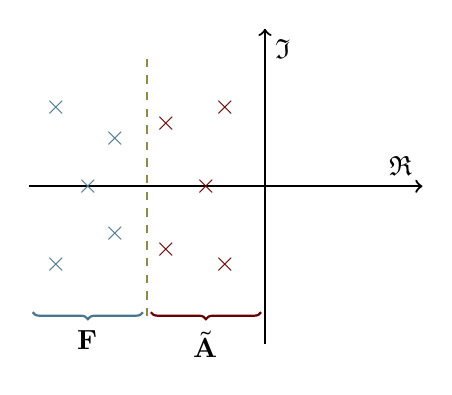
\begin{tikzpicture}[thick]
    \draw[-to] (-3,0) -- (2,0) node[above left] {$\Re$};
    \draw[-to] (0,-2) -- (0,2) node[below right] {$\Im$};

    \draw[darkYellow, dashed] (-1.5, -1.65) -- ++(0, 3.3);
    % Igen ezek szorzásjelek xd
    \node[darkRed] at (-.75, 0) {$\times$};
    \node[darkRed] at (-.5, 1) {$\times$};
    \node[darkRed] at (-.5,-1) {$\times$};
    \node[darkRed] at (-1.25, .8) {$\times$};
    \node[darkRed] at (-1.25,-.8) {$\times$};

    \draw[decorate, decoration={brace}, draw=darkRed]
    (-.05,-1.6) -- (-1.45,-1.6) node[midway, below=1mm] {$\tmat A$};

    \node[darkBlue] at (-2.65, -1) {$\times$};
    \node[darkBlue] at (-2.65, 1) {$\times$};
    \node[darkBlue] at (-2.25,0) {$\times$};
    \node[darkBlue] at (-1.9, .6) {$\times$};
    \node[darkBlue] at (-1.9,-.6) {$\times$};

    \draw[decorate, decoration={brace}, draw=darkBlue]
    (-1.55,-1.6) -- (-2.95,-1.6) node[midway, below=1mm] {$\rmat F$};
  \end{tikzpicture}
  \caption{A rendszer pólusainak elhelyezkedése a komplex számsíkon}
  \label{fig:poles}
\end{figure}


% \backmatter

% \listoffigures
% \listoftables

\end{document}
